% Salvare come: thesis_figures/cap3/multicloud_pattern.tex
% O generare PDF con standalone e includere come multicloud_pattern.pdf
\documentclass[tikz,border=10pt]{standalone}
\usepackage{tikz}
\usetikzlibrary{shapes.geometric,shapes.symbols,arrows,positioning}

\begin{document}
% \begin{figure}[htbp]
% \centering
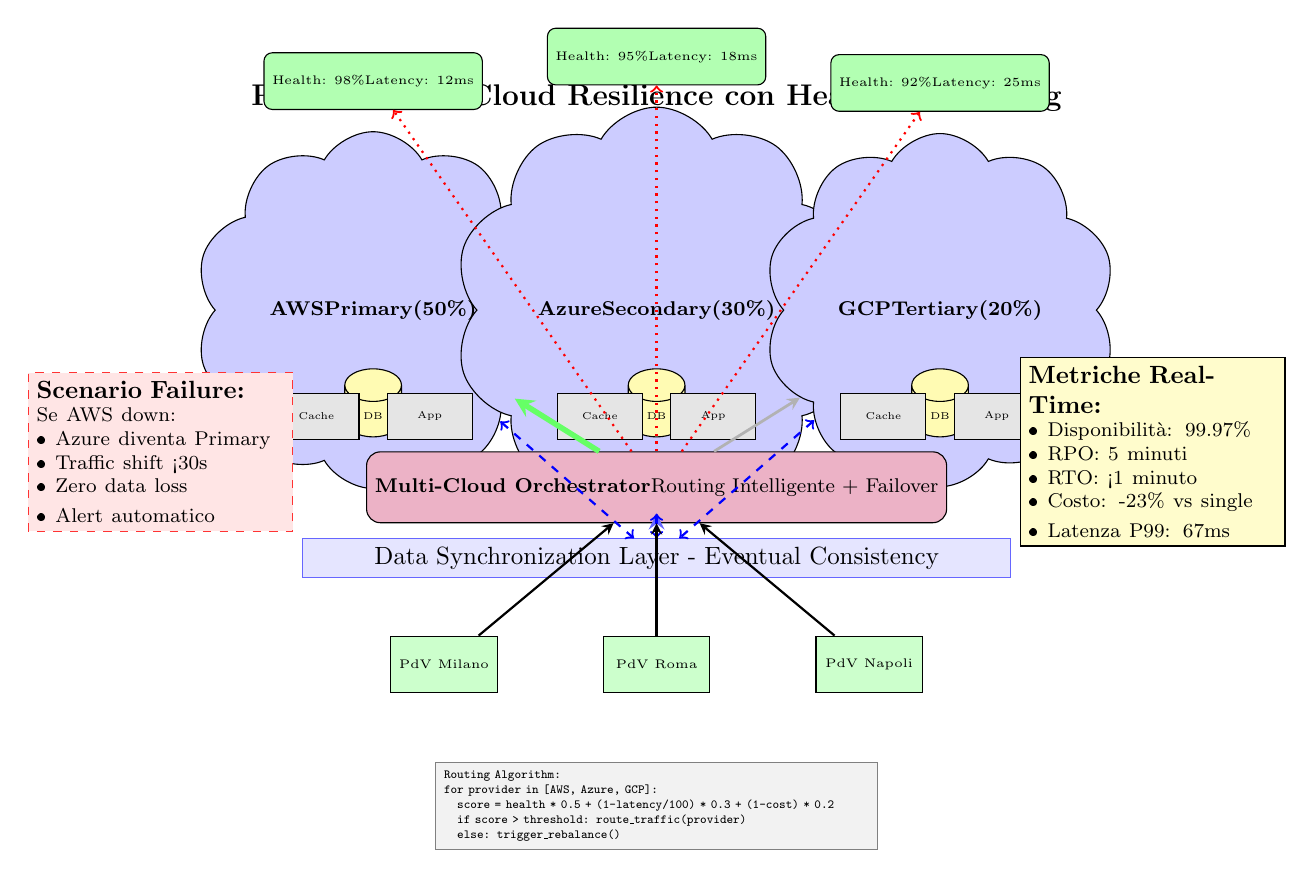
\begin{tikzpicture}[
    scale=0.9,
    transform shape,
    % Stili dei nodi
    cloudprovider/.style={
        cloud, draw, fill=blue!20, 
        cloud puffs=10, cloud puff arc=120, 
        minimum width=3cm, minimum height=2cm,
        font=\footnotesize\bfseries
    },
    loadbalancer/.style={
        rectangle, draw, fill=orange!30,
        minimum width=2.5cm, minimum height=1cm,
        rounded corners=5pt, font=\footnotesize
    },
    monitor/.style={
        rectangle, draw, fill=green!30,
        minimum width=2cm, minimum height=0.8cm,
        rounded corners=3pt, font=\tiny
    },
    store/.style={
        rectangle, draw, fill=gray!20,
        minimum width=1.5cm, minimum height=0.8cm,
        font=\tiny
    },
    database/.style={
        cylinder, draw, fill=yellow!30,
        minimum width=1cm, minimum height=1.2cm,
        shape border rotate=90, font=\tiny
    },
    arrow/.style={->, thick, >=stealth},
    dataarrow/.style={<->, thick, dashed, blue},
    healthcheck/.style={->, dotted, red, thick}
]

% Titolo
\node[font=\large\bfseries] at (0,8) {Pattern Multi-Cloud Resilience con Health Monitoring};

% Cloud Providers
\node[cloudprovider] (aws) at (-4,5) {AWS\\Primary\\(50\%)};
\node[cloudprovider] (azure) at (0,5) {Azure\\Secondary\\(30\%)};
\node[cloudprovider] (gcp) at (4,5) {GCP\\Tertiary\\(20\%)};

% Health Scores
\node[monitor, above=0.3cm of aws] (health1) {Health: 98\%\\Latency: 12ms};
\node[monitor, above=0.3cm of azure] (health2) {Health: 95\%\\Latency: 18ms};
\node[monitor, above=0.3cm of gcp] (health3) {Health: 92\%\\Latency: 25ms};

% Multi-Cloud Orchestrator
\node[loadbalancer, fill=purple!30] (orchestrator) at (0,2.5) {
    \textbf{Multi-Cloud Orchestrator}\\
    Routing Intelligente + Failover
};

% Componenti in ogni cloud
\begin{scope}[shift={(-4,3.5)}, scale=0.8]
    \node[database] (db1) at (0,0) {DB};
    \node[store] (app1) at (1,0) {App};
    \node[store] (cache1) at (-1,0) {Cache};
\end{scope}

\begin{scope}[shift={(0,3.5)}, scale=0.8]
    \node[database] (db2) at (0,0) {DB};
    \node[store] (app2) at (1,0) {App};
    \node[store] (cache2) at (-1,0) {Cache};
\end{scope}

\begin{scope}[shift={(4,3.5)}, scale=0.8]
    \node[database] (db3) at (0,0) {DB};
    \node[store] (app3) at (1,0) {App};
    \node[store] (cache3) at (-1,0) {Cache};
\end{scope}

% Data Synchronization Layer
\node[rectangle, draw=blue!60, fill=blue!10, 
      minimum width=10cm, minimum height=0.5cm] 
    (syncLayer) at (0,1.5) {Data Synchronization Layer - Eventual Consistency};

% Punti Vendita
\node[store, fill=green!20] (pv1) at (-3,0) {PdV Milano};
\node[store, fill=green!20] (pv2) at (0,0) {PdV Roma};
\node[store, fill=green!20] (pv3) at (3,0) {PdV Napoli};

% Connessioni
\draw[arrow, thick, green!60, line width=2pt] (orchestrator) -- (aws);
\draw[arrow, thick, blue!60, line width=1.5pt] (orchestrator) -- (azure);
\draw[arrow, thick, gray!60, line width=1pt] (orchestrator) -- (gcp);

% Health checks
\draw[healthcheck] (orchestrator) -- (health1);
\draw[healthcheck] (orchestrator) -- (health2);
\draw[healthcheck] (orchestrator) -- (health3);

% Data sync
\draw[dataarrow] (aws) -- (syncLayer);
\draw[dataarrow] (azure) -- (syncLayer);
\draw[dataarrow] (gcp) -- (syncLayer);

% Connessioni dai PdV
\draw[arrow] (pv1) -- (orchestrator);
\draw[arrow] (pv2) -- (orchestrator);
\draw[arrow] (pv3) -- (orchestrator);

% Metriche Box
\node[rectangle, draw=black, fill=yellow!20, 
      text width=3.5cm, align=left] at (7,3) {
    \textbf{Metriche Real-Time:}\\
    \footnotesize
    • Disponibilità: 99.97\%\\
    • RPO: 5 minuti\\
    • RTO: <1 minuto\\
    • Costo: -23\% vs single\\
    • Latenza P99: 67ms
};

% Failure Scenario Box
\node[rectangle, draw=red!80, fill=red!10, dashed,
      text width=3.5cm, align=left] at (-7,3) {
    \textbf{Scenario Failure:}\\
    \footnotesize
    Se AWS down:\\
    • Azure diventa Primary\\
    • Traffic shift <30s\\
    • Zero data loss\\
    • Alert automatico
};

% Algoritmo di routing (pseudocodice semplificato)
\node[rectangle, draw=gray, fill=gray!10, 
      text width=6cm, align=left, font=\tiny\ttfamily] at (0,-2) {
    \textbf{Routing Algorithm:}\\
    for provider in [AWS, Azure, GCP]:\\
    \quad score = health * 0.5 + (1-latency/100) * 0.3 + (1-cost) * 0.2\\
    \quad if score > threshold: route\_traffic(provider)\\
    \quad else: trigger\_rebalance()
};

\end{tikzpicture}
% \caption{Pattern Multi-Cloud Resilience con bilanciamento dinamico del carico basato su metriche di salute real-time. Il sistema mantiene repliche attive su 3 cloud provider con sincronizzazione eventual consistency. L'orchestratore monitora continuamente health score, latenza e costi per routing ottimale. In caso di failure di un provider, il traffic shifting avviene in <30 secondi senza perdita di dati.}
% \label{fig:multicloud_pattern}
% \end{figure}
\end{document}
